\section{Methodology}
\label{sec:method}

\subsection{Objective and problem formulation}
\label{sec:objective}

We study supervised reasoning tasks where each training example provides a question $q$,
an optional chain-of-thought $r = (r_1,\dots,r_M)$, and a final answer
$a = (a_1,\dots,a_N)$. We write the full textual sequence as
\[
y \;=\; [\,q \,;\, r \,;\, a\,].
\]
A standard causal language model learns $p_\theta(y)$ and is trained by maximum likelihood.

\paragraph{Goal.}
We seek a model that (i) performs multi-step reasoning using \emph{continuous} internal states
rather than explicit rationale tokens, while (ii) preserving the autoregressive semantics of answer
generation, and (iii) avoiding the \emph{serial} compute overhead incurred when continuous reasoning
is designed as a recurrent unrolling.

\paragraph{Key bottleneck.}
Coconut \cite{hao2024training} demonstrates that replacing parts of the rationale with continuous hidden states can improve
reasoning quality, but it constructs continuous thoughts \emph{sequentially} by feeding the previous
hidden state back as the next input embedding, which enforces a recurrence and introduces a serial
dependence across latent steps. This makes the cost grow linearly with the number of latent steps and
limits hardware parallelism. 

\paragraph{Hypothesis.}
The central hypothesis behind proposed {Parallel Continuous Thought (PaCT)} is that the benefits of
continuous latent reasoning do not require \emph{recurrent} latent unrolling. Instead, following can be carried out 
(i) synthesize a \emph{set} of latent reasoning states in parallel from the current textual context,
(ii) allow rich interaction \emph{within} this latent workspace, and (iii) condition answer decoding on
this workspace under a causal interface. 


\subsection{Preliminaries: causal LMs and Coconut-style latent replacement}
\label{sec:prelims}

\paragraph{Causal transformer LM.}
Let $\mathcal{V}$ be the vocabulary and $d$ the hidden size. A causal LM maps token prefixes
$x_{\le t}=(x_1,\dots,x_t)$ to hidden states $H_t\in\mathbb{R}^{t\times d}$ and next-token probabilities:
\[
\begin{aligned}
H_t &= \mathrm{Transformer}_\theta\!\left(e(x_{\le t})\right), \\
p_\theta(x_{t+1}\mid x_{\le t})
&= \mathrm{softmax}(W h_t).
\end{aligned}
\]




Training minimizes the negative log-likelihood (cross-entropy) over target tokens.

\paragraph{Chain of continuous thought.}
Coconut \cite{hao2024training} replaces a prefix of rationale tokens by \emph{continuous thoughts} that are not decoded as
language. During latent mode, the input embedding at the next latent position is the previous hidden
state, creating a sequential recurrence; the LM loss is masked on latent positions. Training uses a
curriculum that progressively replaces the first $k$ rationale steps by $k\!\times\!c$ continuous thoughts.


\paragraph{Limitation.}
Each continuous thought in Coconut depends on the previous thought, producing $n$ latent
steps requires $n$ serial Transformer invocations along with decoding, which reinstates an RNN-like bottleneck inside a Transformer. 


\subsection{Parallel Continuous Thought (PaCT)}
\label{sec:pact}

\begin{figure*}[h!]
  \centering
  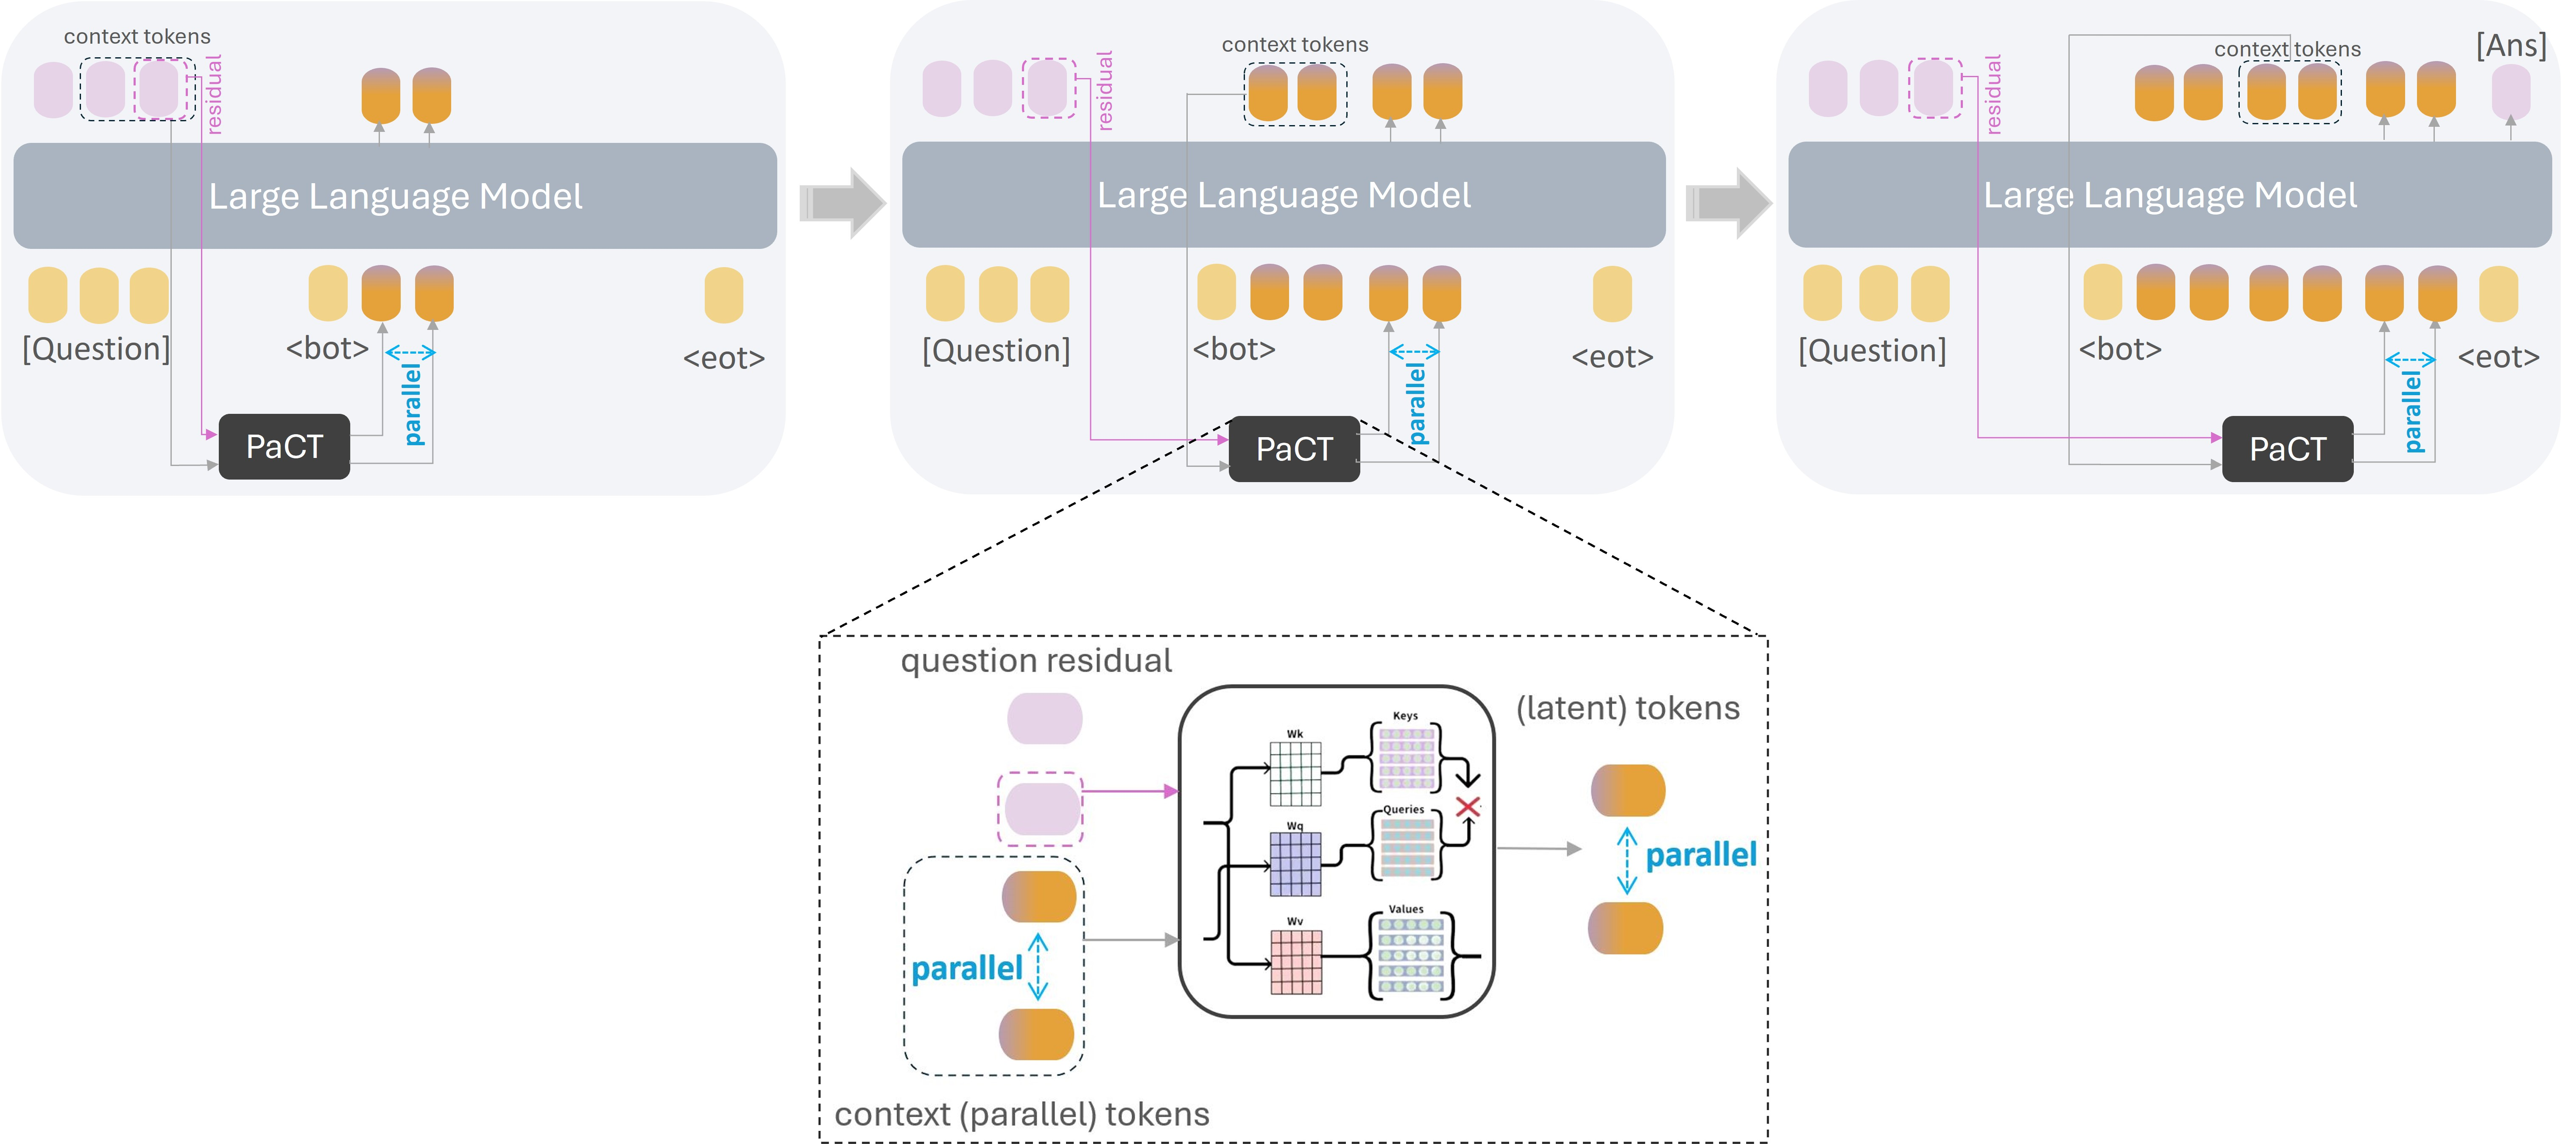
\includegraphics[width=\linewidth]{imgs/parallel_thinking_in_PaCT.jpg}
  %\vspace{2mm}
      \caption{PaCT generates latent tokens in parallel via cross-attention to the textual context, with bidirectional interaction in the latent space}
  \label{fig:PaCT_module}
\end{figure*}

PaCT replaces recurrent latent unrolling with a \emph{parallel latent workspace} updated in
\emph{stages}. Each stage constructs multiple latent vectors simultaneously, refines them via
bidirectional latent interaction, and then exposes them to subsequent token decoding.
Conceptually, one stage performs:

\begin{center}
\begin{tikzpicture}[
    node/.style={
        draw,
        rounded corners,
        inner sep=2pt,
        font=\scriptsize
    },
    arrow/.style={->, thick}
]
\node[node] (e) {\textbf{Text Encoding}};
\node[node, right=4mm of e] (s) {\textbf{Latent Synthesis}};
\node[node, right=4mm of s] (d) {\textbf{Latent Refinement}};
\node[node, right=4mm of d] (c) {\textbf{Decoding}};

\draw[arrow] (e) -- (s);
\draw[arrow] (s) -- (d);
\draw[arrow] (d) -- (c);

\node[below=1mm of e, font=\small] {Causal};
\node[below=1mm of s, font=\small] {Parallel};
\node[below=1mm of d, font=\small] {Bidirectional};
\node[below=1mm of c, font=\small] {Causal};
\end{tikzpicture}
\end{center}




This preserves autoregressive decoding while enabling parallel computation within the latent space.



\subsubsection{Latent capacity: a learnable codebook of query slots}
\label{sec:codebook}
% \begin{figure*}[h!]
%   \centering
%   \includegraphics[width=0.8\linewidth]{imgs/PaCT_module.PNG}
%   \caption{(a) Learnable codebook queries generate latent tokens in parallel via cross-attention to the textual context, with bidirectional interaction in the latent workspace; (b) the attention structure enforces causal text attention while allowing latents to attend to text and earlier latent stages, preserving autoregressive decoding. \textcolor{red}{Prakash, Incorporate suggestions from Prof.}}
%   \label{fig:PaCT_module}
% \end{figure*}


Let $L$ be the number of latent ``slots'' per stage. PaCT maintains a learnable codebook
\[
Q \;=\; \{q_1,\dots,q_L\}, \qquad q_i\in\mathbb{R}^d,
\]
which acts as a persistent set of queries that extract task-relevant summaries from the current
textual state. The codebook defines the \emph{width} of the latent workspace. 

\paragraph{Grounded initialization for stability.}
To anchor the latent workspace to the task specification, we use the question representation as a
shared residual. Let $h_q\in\mathbb{R}^d$ denote the hidden state of the final question token.
We initialize the output projection of the latent synthesis cross-attention to zero and add $h_q$ to
each latent slot after synthesis, so that at initialization all latents start as grounded copies of the
question representation and only deviate when learning discovers useful refinements. 


\subsubsection{Parallel latent synthesis by cross-attention}
\label{sec:latent_synthesis}

Let $H\in\mathbb{R}^{T\times d}$ be the hidden states of the current text prefix (question plus any
remaining rationale tokens). We synthesize latents in one operation using cross-attention with
codebook queries and contextual keys/values.

\paragraph{Context window (causal consistency).}
We optionally restrict keys/values to a recent window $H_{t-k:t}=[h_{t-k},\dots,h_t]$ to enforce that
latent updates depend only on available past information. 

\paragraph{Operator form.}
Denote standard multi-head attention by $\mathrm{Attn}(\cdot)$. Latents are produced as
\[
Z \;=\; \mathrm{CrossAttn}(Q,\;K,\;V), \qquad
K=V=H_{t-k:t},
\]
yielding $Z\in\mathbb{R}^{L\times d}$ computed \emph{in parallel}. This is the first key departure from
Coconut: the number of latent vectors is no longer tied to the number of Transformer invocations.



\subsubsection{Latent refinement via bidirectional self-attention}
\label{sec:latent_deliberation}

\begin{figure}[h]
  \centering
  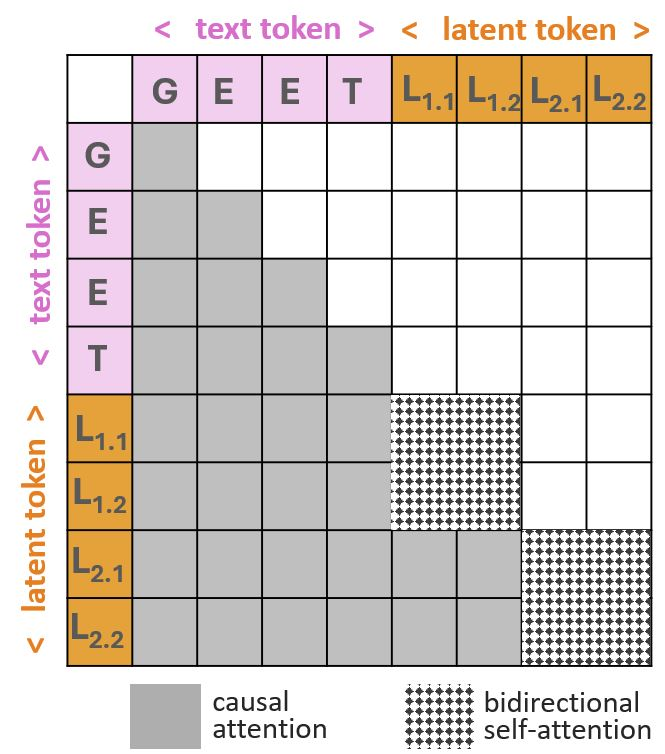
\includegraphics[width=0.6\linewidth]{imgs/bidirectional_self_attention.JPG}
  \caption{Visualizing bi-directional self-attention for latent tokens}
  \label{fig:bidirectional_self_attention}
\end{figure}

After synthesis, the latent slots refine one another within a latent-only workspace. We first ground
each latent by adding the shared question residual:
\[
\tilde{Z} \;=\; Z + \mathbf{1} h_q^\top,
\]
where $\mathbf{1}\in\mathbb{R}^L$ is the all-ones vector. We then apply latent self-attention with a
\emph{bidirectional} mask:
\[
Z' \;=\; \mathrm{SelfAttn}(\tilde{Z}).
\]
Bidirectional interaction is confined to the latent workspace: latents do not attend to future answer tokens, and earlier question tokens do not attend to latents (by causality), ensuring no label leakage while allowing rich coordination among latent hypotheses (Fig. \ref{fig:bidirectional_self_attention}). 
This residual grounding serves two purposes. First, it anchors all latent reasoning vectors to a shared semantic representation of the task specification, ensuring that deliberation remains explicitly conditioned on the question throughout the reasoning process. Second, it bounds the latent update to depend only on the current textual state, rather than the full history of latent computations, thereby reinforcing a Markovian structure in latent reasoning. Each iteration updates the latent state as a function of the current context and a fixed task representation, rather than recursively accumulating unstructured latent history.
%This workspace can be viewed as parallel hypothesis refinement: each slot receives a contextual summary, then exchanges information with other slots before conditioning decoding.


\subsubsection{Conditioning decoding on latents}
\label{sec:conditioning}

We condition subsequent decoding on the latent workspace using a causal interface:
answer tokens may attend to both prior text tokens and the latent slots produced by PaCT.
Concretely, we implement this by \textit{concatenating} latent tokens into the attention context and
adding a \textit{cross-attention pathway} from text representations to latent keys/values.
This matches the intended computation:
\[
p(a \mid q) \;\approx\; p(a \mid q,\; Z'^{(1:S)}),
\]
where $Z'^{(1:S)}$ denotes the latent workspaces across $S$ stages.



\paragraph{Causal mask.}
Let the full sequence ordering be \texttt{[question ; latent stages ; remaining text/answer]}.
We use an attention mask that enforces:
(i) text-to-text remains causal,
(ii) text cannot attend to later latents,
(iii) latents can attend to all previous text and to all latents within their stage bidirectionally,
(iv) answer tokens can attend to all earlier text and all latents.
This realizes the \textit{Text $\rightarrow$ Latents $\rightarrow$ Text} pattern while preserving autoregressive
answer generation. 


\subsubsection{Multi-stage latent reasoning (depth)}
\label{sec:stages}

We repeat the latent workspace construction for $S$ stages, where each stage produces a workspace that conditions subsequent computation. This yields two scaling axes: width $L$ (parallel slots per stage) and depth $S$ (sequential workspace updates). Empirically, increasing depth is more effective than increasing width, consistent with our latent similarity analyses showing redundancy within stages but substantial variation across stages.




\subsection{PaCT training}
\label{sec:training}

\subsubsection{Curriculum schedule}
\label{sec:curriculum}

Like Coconut, we use a curriculum that progressively removes supervised text CoT tokens and
replaces them with latent computation, which stabilizes optimization compared to training purely
from $(q,a)$ pairs. 

Let $m_s$ be the number of rationale steps replaced at curriculum stage $s$.
We construct a training sequence by replacing the first $m_s$ rationale steps with $S_s$ latent stages
(each producing $L$ latent slots). The remaining suffix rationale (if any) and the answer remain as
language tokens for supervision.

\subsubsection{Masked language modeling objective}
\label{sec:loss}

Let $\mathcal{I}_{\text{text}}$ denote indices of \emph{language} tokens (question, remaining rationale,
answer), and let $\mathcal{I}_{\text{lat}}$ denote indices occupied by latent slots. We train by minimizing
\[
\mathcal{L}(\theta) \;=\;
-\sum_{t\in \mathcal{I}_{\text{text}}}
\log p_\theta(x_{t}\mid x_{<t}, Z'^{(1:S)}),
\]
i.e., standard next-token prediction on text tokens, with the loss \emph{masked} on latent positions.
This keeps the learning signal identical in form to standard LM training while allowing latent
computation to be learned implicitly through its effect on answer likelihood. 


% \subsubsection{Algorithm}
% \label{sec:algorithm}
\begin{algorithm}[t]
\caption{Curriculum training for PaCT}
\label{alg:cct_formal}
\begin{algorithmic}[1]
\Require Dataset $\mathcal{D}$, curriculum schedule $\{m_s,S_s\}_{s=0}^{S_{\max}}$, slots $L$, parameters $\theta$, stepsize $\eta$
\For{$s=0,\dots,S_{\max}$}
  \For{$(q,r,a)\sim \mathcal{D}$}
    \State $(\tilde{r}_s,\,\mathcal{M}_s)\leftarrow \mathrm{Replace}(r;\,m_s, S_s, L)$
    \State $x_s \leftarrow [\,q;\ \tilde{r}_s;\ a\,]$
    \State $(\mathbf{p}_\theta(\cdot\mid x_s),\,Z'^{(1:S_s)}) \leftarrow \mathrm{PaCT}_\theta(x_s;\mathcal{M}_s)$
    \State $\mathcal{L}_s(\theta)\leftarrow -\sum\limits_{t\in \mathcal{I}_{\text{text}}(x_s)} \log \mathbf{p}_\theta(x_s[t]\mid x_s[<t],Z'^{(1:S_s)})$
    \State $\theta \leftarrow \theta - \eta \nabla_\theta \mathcal{L}_s(\theta)$
  \EndFor
\EndFor
\end{algorithmic}
\end{algorithm}


\subsection{Computational analysis: removing recurrent latent unrolling}
\label{sec:complexity}

Efficiency is governed by \emph{serial depth} (critical-path length), since parallel hardware can amortize
large matrix multiplications but cannot parallelize a long chain of dependent Transformer invocations.
Let $T$ be the number of causal text decoding steps (tokens for which logits are produced) and
$n_{\text{lat}}$ the number of latent reasoning vectors.

\paragraph{Serial depth.}
In Coconut, latent vectors are generated recurrently ($z_{j+1}$ depends on $z_j$), hence each latent requires
an additional dependent Transformer update:
\[
D_{\text{seq}}^{\textsc{Coconut}} = T + n_{\text{lat}}.
\]
In PaCT, latents are produced in \emph{parallel} within each stage: $L$ latent slots are synthesized by a single
codebook$\rightarrow$text cross-attention and refined by latent-only self-attention. With $S$ stages and
$n_{\text{lat}}=SL$,
\[
D_{\text{seq}}^{\textsc{PaCT}} = T + S,
\qquad\text{so}\qquad
\frac{D_{\text{seq}}^{\textsc{Coconut}}-T}{D_{\text{seq}}^{\textsc{PaCT}}-T}=\frac{n_{\text{lat}}}{S}=L.
\]
Thus, for a fixed latent budget $n_{\text{lat}}$, PaCT reduces the latent-induced serial depth by a factor of $L$.

PaCT shifts computation from a serialized chain to parallel attention/GEMM operations:
per stage, cross-attention over a context window of length $k$ costs $\tilde{O}(Lkd)$ and latent self-attention costs
$\tilde{O}(L^2d)$. Increasing width $L$ therefore increases \emph{parallel work} but does not increase the critical path;
only increasing the number of stages $S$ increases serial depth. This width--depth decoupling is the core computational
advantage of PaCT over recurrent latent unrolling.

%%%%%%%%


%%%%%%%%


%%%%%%%%%%%%
%%%%%%%%%%%%%%%%%%%%%%%%%%%%%%%%%%%%%%%%%%%%%%%%%%%%%%%%%%%%%%%%%%%%%%%